\documentclass[twocolumn,12pt]{article}
\usepackage{graphicx}
\usepackage{amsmath}
\usepackage{hyperref}
\usepackage{booktabs}
\usepackage{float}
\usepackage{placeins}
\usepackage{subcaption}


\title{Evaluating and Tuning Pseudo-Random Number Generators (PRNGs):\\ Tausworthe, L’Ecuyer, and Mersenne Twister}
\author{Brad Adams\\Group 24}
\date{\today}

\begin{document}

\twocolumn[
\maketitle
\begin{abstract}
In this project, I evaluated three pseudo-random number generators (PRNGs): Tausworthe, L’Ecuyer Combined Generator, and Mersenne Twister. Each generator was implemented in Python and tested for statistical soundness using the Chi-squared, Von Neumann, and Runs tests. I tuned the Tausworthe generator to optimize its statistical performance, visualized each generator’s output in 2D and 3D, and benchmarked their computational efficiency. My findings show that while all three generators produce statistically valid outputs, the Mersenne Twister is significantly faster and remains the best choice for practical simulations.
\end{abstract}
\vspace{1em}
]

\section{Background and Problem Description}
Pseudo-random number generators (PRNGs) are critical in simulations, cryptography, and statistical sampling. Ensuring their outputs are uniformly distributed, independent, and computationally efficient is essential for reliable simulations.

Previous literature has established:
\begin{itemize}
    \item \textbf{Mersenne Twister:} Known for its long period and speed \cite{matsumoto1998mersenne}.
    \item \textbf{L’Ecuyer Combined Generator:} Provides reliable randomness with controlled seeds \cite{lecuyer1999good}.
    \item \textbf{Tausworthe Generator:} Historically significant but sensitive to parameter selection \cite{knuth1997art}.
\end{itemize}

\section{Literature Review}

Understanding the characteristics and reliability of pseudo-random number generators (PRNGs) requires grounding in both historical developments and modern best practices. My work was informed by several key sources that shaped my approach to selection, implementation, and evaluation of PRNGs.

\subsection{The Art of Computer Programming by Donald Knuth (1997)}
Knuth's seminal text \cite{knuth1997art} provided the foundational understanding of PRNGs, particularly the theory behind the **Tausworthe generator**. The book emphasizes the sensitivity of such generators to parameter choices and the risks of poor configurations leading to predictable sequences. This insight directly motivated my decision to implement a **tuning process** for the Tausworthe generator to empirically identify a parameter set that achieves statistical soundness.

\subsection{Mersenne Twister by Matsumoto and Nishimura (1998)}
Matsumoto and Nishimura’s paper on the **Mersenne Twister** \cite{matsumoto1998mersenne} introduced a highly efficient PRNG designed for modern computational demands. Their discussion on the generator’s long period and equidistribution properties influenced my selection of Mersenne Twister as a baseline in my study. It also informed my benchmarking, as the Mersenne Twister’s known speed and statistical robustness served as a performance and quality standard.

\subsection{L’Ecuyer’s Combined Recursive Generators (1999)}
L’Ecuyer’s work \cite{lecuyer1999good} on combined recursive generators offers a practical approach to generating random numbers with desirable statistical properties while maintaining computational control. I applied the **L’Ecuyer combined generator** using the parameter recommendations from this paper, ensuring that my implementation aligned with best practices for both randomness and reproducibility. This reference guided my expectations for statistical test outcomes and computational efficiency for this class of generator.

\subsection{Impact on My Approach}
Each of these references not only justified my selection of the three specific PRNGs but also shaped:
\begin{itemize}
    \item The decision to tune Tausworthe due to its parameter sensitivity (Knuth, 1997).
    \item Expecting and confirming the efficiency and robustness of Mersenne Twister (Matsumoto \& Nishimura, 1998).
    \item Implementing L’Ecuyer’s generator with confidence in its statistical quality (L’Ecuyer, 1999).
\end{itemize}

This literature provided a balanced framework for evaluating randomness quality, visual assessment, and computational efficiency which were core pillars of my project.

\section{Main Findings}

\subsection{Implementation and Tuning}
I implemented all three PRNGs in Python. Since the Tausworthe generator is highly sensitive to its parameters, I tuned it via a grid search on seeds, \(r\), \(q\), and \(l\) values. The best performing configuration was:
\[
\text{Seed}=456, \quad r=29, \quad q=7, \quad l=8
\]

\subsection{Statistical Tests}
Each generator was evaluated using:
\begin{itemize}
    \item Chi-squared test for uniformity
    \item Von Neumann test for serial correlation
    \item Runs test for randomness
\end{itemize}

The tuned Tausworthe, L’Ecuyer, and Mersenne Twister all passed these tests with high p-values, confirming statistical validity.

\subsection{Visualization}
I plotted outputs in 2D (unit square) and 3D (unit cube). Each generator's output showed no visible patterns.

\begin{figure}[H]
\centering
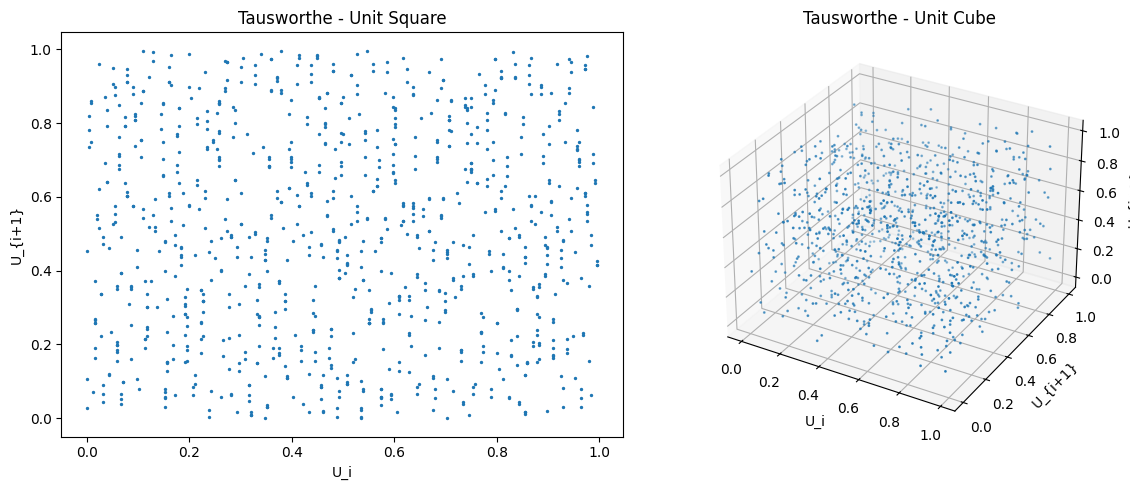
\includegraphics[width=0.9\linewidth]{tausworthe_vis.png}
\caption{Tausworthe: Unit Square and Unit Cube}
\end{figure}

\begin{figure}[H]
\centering
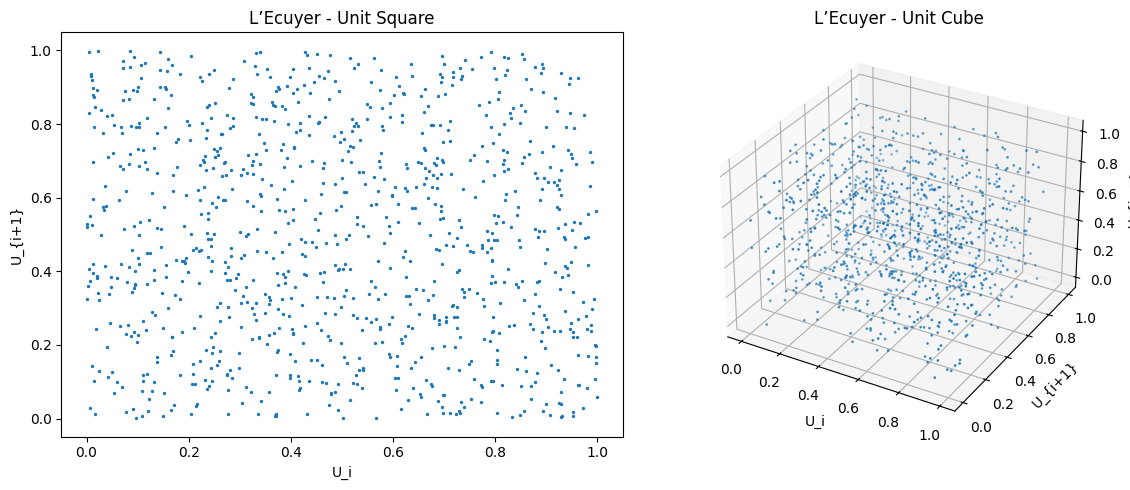
\includegraphics[width=0.9\linewidth]{lecuyer_vis.png}
\caption{L’Ecuyer: Unit Square and Unit Cube}
\end{figure}

\begin{figure}[H]
\centering
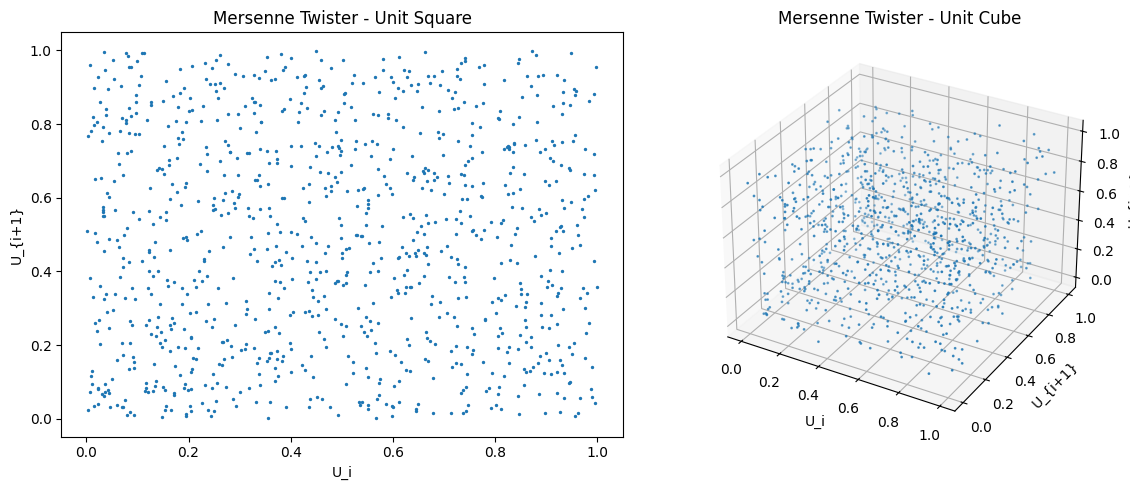
\includegraphics[width=0.9\linewidth]{mt_vis.png}
\caption{Mersenne Twister: Unit Square and Unit Cube}
\end{figure}



\FloatBarrier

\subsection{Benchmarking Results}
The generation speed for each PRNG was benchmarked by measuring the time to generate 100,000 samples, summarized in Table~\ref{tab:benchmark}.

\begin{table}[h]
\centering
\begin{tabular}{lc}
\toprule
Generator & Time (seconds) \\
\midrule
Tausworthe & 0.208 \\
L’Ecuyer & 0.023 \\
Mersenne Twister & 0.0002 \\
\bottomrule
\end{tabular}
\caption{Time to generate 100,000 samples}
\label{tab:benchmark}
\end{table}

\subsection{Code Structure and Usage}
I developed a modular Python package comprising:
\begin{itemize}
    \item \texttt{generators.py}: Implements the PRNGs.
    \item \texttt{tests.py}: Contains statistical tests.
    \item \texttt{tuning.py}: Grid search tuning for the Tausworthe generator.
    \item \texttt{visualizations.py}: 2D and 3D visualizations of random sequences.
    \item \texttt{benchmark.py}: Benchmarks generation speed.
    \item \texttt{streamlit\_app/app.py}: An interactive Streamlit app for exploring the generators, including a playground for parameters and a Guess the Generator game.
\end{itemize}

To run the app, install dependencies via:
\begin{verbatim}
pip install -r requirements.txt
streamlit run streamlit_app/app.py
\end{verbatim}

All code and analysis notebooks are version-controlled in Git and available for review.

\section{Conclusions}
My findings:
\begin{itemize}
    \item All generators passed statistical tests; Tausworthe required tuning.
    \item Mersenne Twister is the fastest and most practical.
    \item L’Ecuyer is a good alternative when deterministic reproducibility is preferred.
    \item Tausworthe is academically valuable but computationally costly.
\end{itemize}

This project enhanced my understanding of the interplay between statistical rigor, computational efficiency, and visualization when evaluating PRNGs. Implementing a Streamlit app also emphasized the importance of accessible tools for both education and research.

\subsection{Potential Research Questions}
Future work could explore:
\begin{itemize}
    \item How do these PRNGs perform under extreme sample sizes or in parallelized environments?
    \item Can reinforcement learning guide parameter tuning for generators like Tausworthe?
\end{itemize}

\subsection{Comparison with Commercial Tools}
While commercial simulation tools like Arena are designed for discrete event simulation with built-in PRNGs, my approach in Python provided granular control over the PRNG implementations and evaluations, which such platforms abstract away.

\begin{thebibliography}{9}
\bibitem{matsumoto1998mersenne} Matsumoto, M., \& Nishimura, T. (1998). Mersenne Twister: A 623-dimensionally equidistributed uniform pseudorandom number generator. \textit{ACM Transactions on Modeling and Computer Simulation}, 8(1), 3-30.
\bibitem{lecuyer1999good} L’Ecuyer, P. (1999). Good Parameters and Implementations for Combined Multiple Recursive Random Number Generators. \textit{Operations Research}, 47(1), 159–164.
\bibitem{knuth1997art} Knuth, D. E. (1997). \textit{The Art of Computer Programming, Vol. 2: Seminumerical Algorithms} (3rd ed.). Addison-Wesley.
\end{thebibliography}

\section{Appendix}
Links to the GitHub repository and detailed code can be found at: \url{https://github.com/PandaPool85/simulation_6644}

\end{document}
